\section{Aufgabe 2: Ensemblemethoden}
\begin{table}[h]
	\begin{tabular}{|l|llll|}
		\hline
		& Entscheidungsbaum & AdaBoost & Random Forest & Bagging \\ \hline
		n\_estimators               &               &        100*          &   100    & \textbf{100}*    \\
		criterion                   &      gini         &            gini       &   gini       & entropy* \\
		max\_depth                  &    \textbf{5}*           &          \textbf{20}*          &    None      & 10*      \\
		min\_samples\_split         &     40*          &      2            &    \textbf{5}*      & 20*      \\
		min\_samples\_leaf          &     100*         &        1           &    1       & 10*      \\
		min\_weight\_fraction\_leaf &   0           &     0              &    0       & 0       \\
		max\_features               &         25*      &          None         &   5*       & 20*      \\
		max\_leaf\_nodes            &       None        &       None            &    None      & None     \\
		min\_impurity\_decrease     &     0          &       0            &    0      & 0     \\
		min\_impurity\_split        &        0.1*       &           0        &     0     & 0.1*     \\ \hline
	\end{tabular}
	\caption{\label{table:gridsearch} Optimale Hyperparameter-Einstellung pro Modell durch die univariate \emph{Grid Search}}
\end{table}

Im Folgenden Abschnitt wird die Implementierung und Optimierung verschiedener Ensemblemethoden und eines Entscheidungsbaums mit Hilfe der \emph{scikit-learn} Bibliothek beschrieben. Um einen Vergleich zwischen verschiedenen Ensemblemethoden herstellen zu können wurde das \emph{Bagging}- und \emph{AdaBoost}-Verfahren, sowie ein \emph{Random-Forest} implementiert. Alle drei \emph{Ensemblemethoden} wurden mit einem Klassifizierungsbaum als Basisklassifizierer erstellt. Die Klassifizierungsgenauigkeit der einzelnen Verfahren mit Standardeinstellungen, sowie nach einer Hyperparameter-Optimierung können in Tabelle \ref{table:results_grid} gefunden werden. 

\subsection{Hyperparameter Optimierung}
Um eine optimale Einstellung der Hyperparameter pro Verfahren zu finden, wurde mit Hilfe der \emph{scikit-learn} Bibliothek das \emph{Grid Search}-Verfahren implementiert. Im Gegensatz zu dem \emph{Random Search}-Verfahren, dass in Kapitel \ref{nn_hyperparams} verwendet wurde, sucht \emph{Grid Search} allen möglichen Hyperparameter-Kombinationen in einem gegebenen Parameterraum.  Als Metrik für die Optimierung wurde auf Grund der einfachen Interpretierbarkeit die Klassifizierungsgenauigkeit (engl. \emph{Accuracy}) gewählt.

\subsubsection{Univariat}
\label{section:univariat}
%TODO: Beschreibung wegen erweiterung des Parameterraums, falls das Optimum das maximum oder minimum des Raumes dargestellt hat.
Die aus der Aufgabenstellung angegebenen Hyperparameter wurden zunächst einzeln (univariat) variiert, um nach einem optimalen Wert pro Hyperparameter zu suchen. Pro Hyperparameter wird also ein einzelner Parameterraum definiert. Hierbei wurde die Suche in zwei Durchläufen durchgeführt. Der Hyperparameter, durch dessen Konfiguration weg von seiner Standardeinstellung, die größte positive Auswirkung auf die Klassifizierungsgenauigkeit erzielt werden konnte, wurde für den  nächsten Durchgang fest konfiguriert und aus dem zu suchenden Parameterraum entfernt. Die Ergebnisse der \emph{Grid Search} pro Modell und Hyperparameter sind in Tabelle \ref{table:gridsearch} dargestellt. Die \textbf{fett} geschriebenen Werte wurden jeweils nach dem Ersten der beiden \emph{Grid Search} Durchläufe festgelegt. Die Werte, die mit * gekennzeichnet sind, weichen von den Standardeinstellungen ab. Zu beachten ist, dass der Hyperparameter \emph{n\_estimators} durch eingeschränkte Rechenkapazitäten auf ein oberes Limit von 100 begrenzt wurde. Eine vollständige Auflistung der durchsuchten Parameterräume pro Hyperparameter ist in Tabelle \ref{table:parameter_grid_univariat} im Anhang zu finden.

In Abbildung \ref{fig:grid_search_max_depth_tree} ist  beispielhaft der erste Durchlauf einer \emph{Grid Search} nach dem Hyperparameter \emph{max\_depth} dargestellt. Es ist zu sehen, dass das \emph{Bagging}-Verfahren, sowie der \emph{Random Forest} robuster gegenüber einer Überanpassung an die Trainingsdaten sind. Zu beachten ist, dass die in der Abbildung dargestellten Kurven auf den Train- und Testdaten aus der 10-fachen Kreuzvalidierung basieren. 

%TODO: Testdaten bei cross validation.
\begin{figure}[ht]
	\centering
	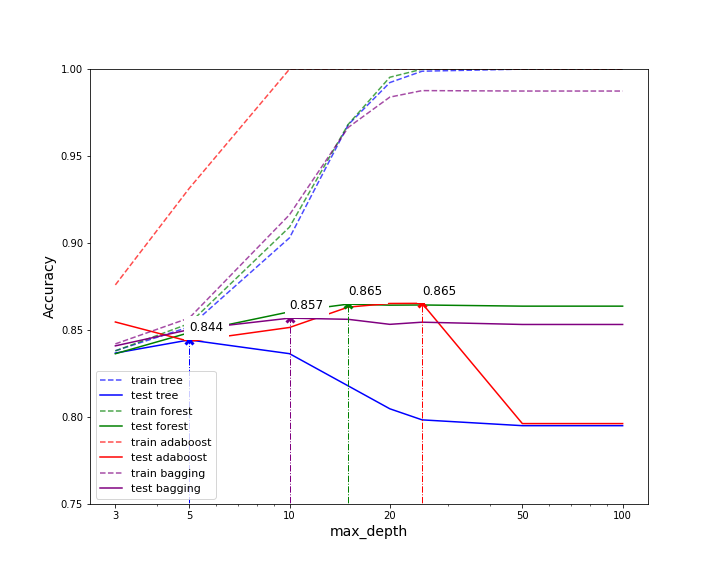
\includegraphics[width = 0.9\textwidth]{Bilder/grid_search_max_depth.png}
	\caption{Klassifizierungsgenauigkeit abhängig des Hyperparameters \emph{max\_depth}}
	\label{fig:grid_search_max_depth_tree}
\end{figure}

 
\subsubsection{Multivariat}
Im Gegensatz zu Abschnitt \ref{section:univariat} werden im folgenden Parameterräume definiert, die mehr als einen Hyperparameter umfassen. Somit können auch optimale Kombinationen von Hyperparameter-Einstellungen untersucht werden. Hierbei sollte darauf geachtet werden, dass die Rechenzeit einer \emph{Grid Search} exponentiell mit der Größe des Parameterraums ansteigt. Demnach werden folgende Hyperparameter von der Suche ausgeschlossen: \emph{n\_estimators}, \emph{min\_samples\_leaf}, \emph{criterion}, \emph{min\_weigh\_fraction\_leaf}, \emph{max\_leaf\_nodes} und \emph{min\_impurity\_split}. Die gewählten Parameterräume, sowie die gewählte Einstellung pro Hyperparameter ist in Tabellen \ref{table:parameter_grid_multivariat_forest} - \ref{table:parameter_grid_multivariat_bagging} im Anhang zu finden. Die Klassifizierungsergebnisse, der durch die multivariate \emph{Grid Serach} optimierten Verfahren, können in Tabelle \ref{table:results_grid} gefunden werden.

\subsubsection{Ergebnisse}
Die Klassifizierungsergebnisse der Verfahren mit Standard Einstellungen, sowie nach einer multivariaten und univariaten \emph{Grid Search} sind in Tabelle \ref{table:results_grid} zu finden. Wie der Tabelle entnommen werden kann, konnten die besten Klassifizierungsergebnisse mit der zweistufigen univariaten \emph{Grid Search} erzielt werden. Die Ergebnisse der Verfahren, die durch die multivariate \emph{Grid Search} optimiert wurden, können wahrscheinlich mit einer Erweiterung des Parameterraums verbessert werden. Dies würde jedoch auf der eingesetzten Hardware zu einem starken Anstieg der Berechnungsdauer führen. Als Alternative für weitergehende Untersuchungen könnte das in Abschnitt \ref{nn_hyperparams} eingesetzte \emph{Random Search} Verfahren angewendet werden.

\begin{table}[h]
	\begin{tabular}{lllll}
		\hline
		& Entscheidungsbaum & AdaBoost & Random Forest & Bagging \\ \hline
		Default Einstellungen         &    79.07\%               &  78,64\%        &  86,36\%             &  85,67\%       \\
		Nach zweistufiger\\
		univariater \emph{Grid Search}   &  84.77\%              &  86,64\%        &        86,43\%       &    86,13\%     \\
		Nach multivariater \emph{Grid Search} &  84,53\%                 &  86,64\%      &   86,34\%              &    85,97\%     \\ \hline
	\end{tabular}
	\caption{\label{table:results_grid} Klassifizierungsgenauigkeiten der Ensemblemethoden vor und nach der Optimierung durch \emph{Grid Search}}
\end{table}



